%%%%%%%%%%%%%%%%%%%%%%%%%%%%%%%%%%%%%%%%%%%%%%%%%%%%%%%%%%%%%%%%%%%%%%%%%%%%
%
%		Relazione sull'assignment n'2 Ping Pong protocol
%
%				    Nicola Corti - 2013
%
%%%%%%%%%%%%%%%%%%%%%%%%%%%%%%%%%%%%%%%%%%%%%%%%%%%%%%%%%%%%%%%%%%%%%%%%%%5%
\documentclass[a4paper,11pt]{article} 
\usepackage{graphicx}
\usepackage{vmargin}
\usepackage[italian]{babel} 
\usepackage[utf8x]{inputenc}
\usepackage{listings}
\usepackage{url}
\usepackage{pdflscape}
\usepackage{hyperref}
\usepackage{tabularx}
\usepackage[usenames,dvipsnames,svgnames,table]{xcolor}

\newcolumntype{P}[1]{>{\raggedright\arraybackslash}p{#1}}


\lstset{
basicstyle=\small\ttfamily,
keywordstyle=\color{MidnightBlue}\bfseries,
identifierstyle=\color{Black},
commentstyle=\color{Green}\itshape,
stringstyle=\color{Red}\ttfamily,
showstringspaces=false,
%numbers=left, numberstyle=\tiny,
%stepnumber=1, numbersep=10pt,
tabsize=4,
framexleftmargin=5mm, rulesepcolor=\color{Gray},
frame=tb,
backgroundcolor=\color{LightGray},
language={Java},
%mathescape=true,
%fontadjust=true,
%breaklines=true,breakatwhitespace=true,breakautoindent
}


\title{Protocollo PING/PONG - Esempio di implementazione in Java}
\author{Nicola Corti - 454413 \\Corso di Laurea Magistrale in Informatica - Universit\`a di pisa}
\date{22 Dicembre 2013}

\renewcommand\lstlistingname{Codice}
\renewcommand\figurename{Immagine}
 
\begin{document}
\maketitle
 
\begin{abstract}
Questa breve relazione ha lo scopo di illustrare i dettagli relativi  alla realizzazione e all'uso di \textsf{PingPong}: un software che simula il comportamento del protocollo Ping/Pong di Gnutella, con o senza il meccanismo di \emph{pong caching}.
\end{abstract}

\tableofcontents

\section*{Introduzione}

\section{Design \& Implementazione}
\label{sec:design}

%%%%% TODO

\subsection{Classe per la gestione dei Messaggi}

La prima classe che occorre descrivere \`e senza dubbio la classe \textsf{Message}, questa classe rappresenta infatti i messaggi che vengono scambiati fra i peer.

Si \`e cercato di realizzare la struttura struttura dei messaggi in modo che fosse quanto pi\`u fedele alla struttura definita nella RFC di Gnutella. Sono stati quindi definiti i seguenti membri:

\begin{description}
\item[\textsf{funcion}] Un campo di tipo \textsf{MessType} (un \textsf{enum}) che pu\`o assumere valore \textsf{PONG} o \textsf{PING} e che rappresenta il tipo del messaggio,
\item[\textsf{GUID}] L'identificatore univoco del messaggio, generato in modo da concatenare il nome del peer che ha generato il messaggio al timestamp di generazione del messaggio,
\item[\textsf{HOP}] Numero di hop che ha effettuato il messaggio,
\item[\textsf{TTL}] \emph{Time-to-leave} ovvero il numero di hop che pu\`o ancora effettuare il messaggio prima di essere scartato dalla rete,
\item[\textsf{sender}] Peer che ha generato il messaggio,
\item[\textsf{lastpeer}] Ultimo peer che ha effettuato il routing del messaggio,
\item[\textsf{sharedbytes}] Numero di byte condivisi dal peer che ha generato il messaggio,
\item[\textsf{sharedfiles}] Numero di file condivisi dal peer che ha generato il messaggio.
\end{description}

La classe offre inoltre alcuni costruttori per generare nuovi messaggi e per impostare correttamente tutti i campi. \`E inoltre presente un \emph{copy constructor} (\textsf{Message(Message m)}) che crea una copia di un messaggio, utile quando un peer deve inviare un messaggio a tanti peer differenti, in modo da evitare conflitti sulle modifiche delle informazioni del messaggio (\textsf{lastpeer}, \textsf{HOP}, etc...).

\subsection{Classi per la realizzazione dei \textsf{Peer}}

Per realizzare il software \`e stata definita una gerarchia di classi che permettono di rappresentare il comportamento di ogni tipo di Peer. La gerarchia delle classi \`e rappresentata nel diagramma delle classi UML in figura \ref{img:uml}

\begin{figure}[ht]
\centering
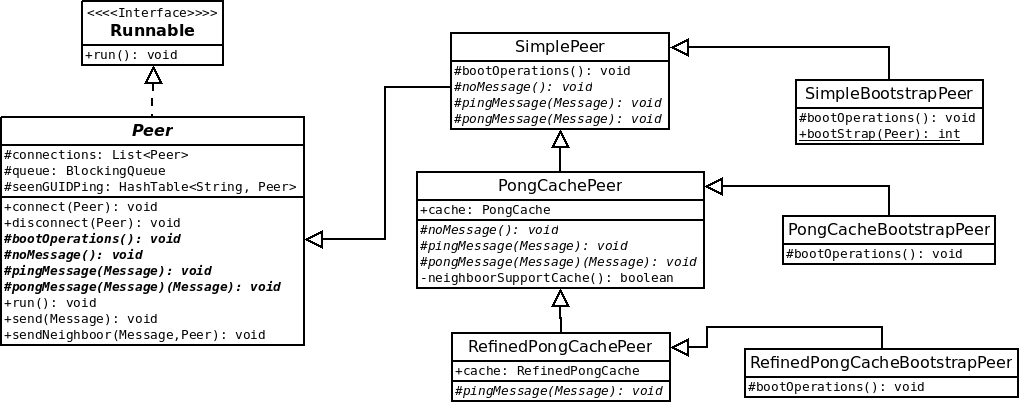
\includegraphics[height=5.7cm]{peers.png}
\caption{\small{Gerarchia delle classi di \textsf{Peer}}}
\label{img:uml}
\end{figure}

La radice della gerarchia \`e rappresentata dalla classe \textsf{Peer}, la classe in questione \`e astratta e contiene dei metodi che devono essere implementati dalle sottoclassi. Le varie sottoclassi della gerarchia contengono il codice per realizzare la logica dietro ogni tipo di peer. Le varie classi verranno presentate in dettaglio nei paragrafi seguenti.

\subsubsection{\textsf{Peer}}

La classe \textsf{Peer} contiene i metodi utili ad ogni tipo di peer. In particolare contiene i seguenti membri:

\begin{description}
\item[\textsf{address}] Una stringa che rappresenta l'indirizzo del peer,
\item[\textsf{connection}] Una lista di oggetti di tipo \textsf{Peer} che rappresenta la lista delle connessioni del peer,
\item[\textsf{queue}] Una \textsf{BlockingQueue} che viene utilizzata per gestire la coda dei messaggi in entrata ad ogni peer. L'oggetto \`e \emph{syncronized} e non crea problemi per quanto riguarda la concorrenza, offre inoltre metodi che sono bloccanti nel caso in cui non vi siano messaggi nella coda e risulta quindi l'ideale per modellare il comportamento dei peer,
\item[\textsf{seenGUIDPing}] Una \textsf{HastTable} per salvare i messaggi di Ping che sono passati, in coppia con il peer che li ha inviati, in modo da poter, realizzare il meccanismo del \emph{backward routing}.
\item[\textsf{PING\_COUNTER}] Un contatore per memorizzare il numero di Ping che sono passati,
\item[\textsf{PONG\_COUNTER}] Un contatore per memorizzare il numero di Pong che sono passati.
\end{description}

Contiene inoltre i seguenti metodi di utilit\`a per ogni tipo di peer:

\begin{description}
\item[\textsf{connect}] Per connettere due peer fra di loro, le connessioni sono bidirezionali ed \`e sufficiente invocare connect sul peer \textsf{A} verso il peer \textsf{B} per connettere \textsf{B} verso \textsf{A} a sua volta,
\item[\textsf{disconnect}] Per disconnettere due peer fra di loro,
\item[\textsf{isconnected}] Per controllare se due peer sono connessi fra di loro,
\item[\textsf{send}] Per inviare un messaggio al peer su cui viene invocato (il messaggio viene accodato nella \textsf{BlockingQueue}),
\item[\textsf{sendNeighboor}] Per inviare un messaggio a tutti i vicini del peer su cui viene invocato.
\end{description}

Inoltre la classe \textsf{Peer} contiene il metodo \textsf{run}\footnote{Implementato dall'interfaccia \textsf{Runnable}}, che risulta essere un metodo fondamentale per l'esecuzione del comportamento dei peer. 


Il metodo \textsf{run} contiene lo ``scheletro'' dell'esecuzione dei peer: il peer si avvia, esegue la funzione \textsf{bootOperations()}; dopo si mette in attesa di un messaggio sulla coda, se non riceve un messaggio entro un certo lasso di tempo esegue la funzione \textsf{noMessage()}, se riceve un messaggio di ping esegue \textsf{pingMessage()}, se invece riceve un messaggio di pong esegue \textsf{pongMessage()}.

Ovviamente le funzioni \textsf{bootOperations()}, \textsf{noMessage()}, \textsf{pingMessage()} e \textsf{pongMessage()} sono funzioni astratte, devono essere implementate dalle sottoclassi.

Con una implementazione di questo genere si svincolano le sottoclassi da dover realizzare tutte le operazioni collegate alla \textsf{BlockingQueue}, in modo da dover implementare solamente la ``business logic'' del peer, ovvero le operazioni legate alla ricezione di messaggi di ping, pong, etc...

\subsubsection{\textsf{SimplePeer}}

La classe \textsf{SimplePeer} rappresenta un'implementazione di \textsf{Peer} che non utilizza il \emph{pong caching}.

La classe \textsf{SimplePeer} implementa i metodi seguenti:
\begin{description}
\item[\textsf{bootOperations}] Non effettuando nulla,
\item[\textsf{noMessage}] Non effettuando nulla,
\item[\textsf{pingMessage}] Salvando nel \textsf{seenGUIDPing} il ping che \`e stato ricevuto, propagandolo a tutti i vicini e generando un messaggio di Pong come risposta,
\item[\textsf{pongMessage}] Cercando nel \textsf{seenGUIDPing} il peer che aveva inviato il ping in passato, in modo da potergli inviare il pong ricevuto (cosidetto meccanismo di \emph{backward routing}).
\end{description}

\subsubsection{\textsf{SimpleBootstrapPeer}}

La classe \textsf{SimpleBootstrapPeer} rappresenta una sottoclasse di \textsf{SimplePeer} che si comporta in modo analogo, tranne per il fatto che esegue la fase di bootstrap.

La classe \textsf{SimpleBootstrapPeer} implementa i metodi seguenti:
\begin{description}
\item[\textsf{bootOperations}] Invocando la funzione statica \textsf{bootStrap},
\item[\textsf{bootStrap}] Funzione statica per effettuare  il bootstrap di un nodo: genera un messaggio di Ping e lo invia al primo peer nella lista dei peer connessi, attende dei pong di risposta per un certo lasso di tempo ed effettua la connessione con i peer in questione.
\end{description}

\subsubsection{\textsf{PongCachePeer}}

La classe \textsf{PongCachePeer} rappresenta una sottoclasse di \textsf{SimplePeer} e si tratta di un peer che utilizza il meccanismo di \emph{pong caching} semplice.

La classe ha un membro \textsf{cache} di tipo \textsf{PongCache} per gestire la cache dei messaggi di pong ricevuti.

La classe \textsf{PongCachePeer} implementa i metodi seguenti:
\begin{description}
\item[\textsf{pingMessage}] Controlla se ci sono pong a sufficienza nella cache per effettuare una risposta tramite la cache, se s\`i risponde con i pong della cache, altrimenti si comporta come \textsf{pingMessage} della superclasse (\textsf{SimplePeer}).
\item[\textsf{pongMessage}] Salva il pong nella cache e si comporta come \textsf{pongMessage} della superclasse (\textsf{SimplePeer}).
\item[\textsf{noMessage}] Invia un messaggio di Ping a tutti i vicini in modo da poter fare il \emph{refresh} delle cache.
\item[\textsf{neighboorSupportCache}] Per controllare se i Ping vicini supportano il \emph{pong caching}. Se infatti i vicini non supportassero il \emph{pong caching} la frequenza con cui vengono mandati i messaggi di ping viene ridotta. 
\end{description}

\subsubsection{\textsf{PongCacheBootstrapPeer}}

La classe \textsf{PongCacheBootstrapPeer} rappresenta una sottoclasse di \textsf{PongCachePeer} che si comporta in modo analogo, tranne per il fatto che esegue la fase di bootstrap.

La classe \textsf{PongCacheBootstrapPeer} implementa il metodo \textsf{bootOperations} invocando la funzione statica \textsf{bootStrap} della classe \textsf{SimpleBootstrapPeer}. 

Si assume infatti che la fase di bootstrap sia analoga per tutti i tipi di peer, appena terminata la fase di bootstrap i peer si comportano come i peer della superclasse (in questo caso \textsf{PongCacheBootstrapPeer} si comporter\`a come un \textsf{PongCachePeer} appena terminata la fase di bootstrap).

\subsubsection{\textsf{RefinedPongCachePeer}}

La classe \textsf{RefinedPongCachePeer} rappresenta una sottoclasse di \textsf{PongCachePeer} e si tratta di un peer che utilizza il meccanismo di \emph{refined pong caching}.

La classe \`e simile alla classe \textsf{PongCachePeer}  tranne per il fatto che il membro \textsf{cache} \`e di tipo \textsf{RefinedPongCache}.

La classe \textsf{RefinedPongCache} implementa il metodo \textsf{pingMessage} rimuovendo dalla cache i ping scaduti e comportandosi come \textsf{pingMessage} della superclasse.

\subsubsection{\textsf{RefinedPongCacheBootstrapPeer}}

La classe \textsf{RefinedPongCacheBootstrapPeer} rappresenta una sottoclasse di \textsf{RefinedPongCachePeer}.

Per questa classe valgono i discorsi analoghi fatti per la classe \textsf{PongCacheBootstrapPeer}

\subsection{Classi per la gestione della \emph{pong cache}}

Per supportare il meccanismo di \emph{pong caching} \`e stato necessario definire due classi: \textsf{PongCache} e \textsf{RefinedPongCache} che gestiscono la cache dei pong nel caso semplice e \emph{refined}.

In particolare la classe \textsf{PongCache} salva i pong all'interno di una \textsf{HashTable} ed offre dei semplici metodi per aggiungere e rimuovere pong:

\begin{description}
\item[addEntry] Per aggiungere un messaggio alla cache (nel caso in cui fosse gi\`a presente un pong pi\`u vecchio proveniente dallo stesso peer questo viene aggiornato),
\item[containsEnough] Per controllare se la cache contiene un numero di pong sufficiente a permettere di rispondere senza trasmettere il ping,
\item[getPongs] Ritorna una lista di pong da poter mandare come risposta al ping ricevuto come parametro,
\item[removeAll] Per rimuovere tutti i pong dalla cache.
\end{description}

La classe \textsf{RefinedPongCache} aggiunge il metodo \textsf{removeExpired} per rimuovere i pong che sono scaduti.

\subsection{Classe per la gestione della rete dei Peer}

La classe che si occupa di gestire la rete dei peer \`e la rete \textsf{PingPongNet}. In particolare si \`e deciso di implementare i peer utilizzando i \textsf{Thread} di Java (si nota infatti che tutte le classi implementano l'interfaccia \textsf{Runnable}).

La classe in particolare si occupa di aggiungere peer di tutti i tipi alla rete, di connetterli, di generare il relativo \textsf{Thread} e di conservarlo in una lista. Una volta invocata la funzione \textsf{start} tutti i thread nella lista vengono avviati.

La classe si occupa anche di effettuare la stampa delle statistiche dei \textsf{Peer} leggendo i contatori \textsf{PING\_COUNTER} e \textsf{PONG\_COUNTER} dai Peer al fine di poter apprezzare le differenze fra le performance delle varie implementazioni.

\subsection{Parametri del Sistema}

Il sistema necessita di una serie di parametri che influenzano fortemente il comportamento del sistema.
Tutti i parametri sono definiti come membri statici della classe \textsf{Par} e sono presentati nella tabella \ref{tab:par}.

\begin{table}
\centering
\begin{tabular}{|P{3.5cm}|P{10cm}|}
\hline
\textbf{Nome} & \textbf{Descrizione} \\
\hline
\textsf{MAIN\_POLL} \textsf{\_STATS\_SECONDS} & Secondi ogni quanto si desidera che il thread \textsf{Main} stampi le statistiche sul sistema \\
\hline
\textsf{MESSAGE} \textsf{\_MAX\_TTL} & Valore massimo del TTL del messaggio. Abbassando il valore si dimunisce il numero di peer che un messaggio pu\`o raggiungere. Il valore deve essere sempre $>= 2$  \\
\hline
\textsf{PEER\_POLL} \textsf{\_SECONDS} & Numero di secondi che un peer deve stare in attesa di un messaggio, dopo questi secondo il peer esegue la funzione \textsf{noMessage} se non ha ricevuto messaggi  \\
\hline
\textsf{BOOTSTRAP} \textsf{\_NEIGHBOOR} \textsf{\_PONG\_PEER} & Parametro utilizzato dai peer che effettuano il bootstrap, rappresenta il numero di peer che si spera di riuscire a contattare nella fase di bootstrap  \\
\hline
\textsf{BOOTSTRAP} \textsf{\_NEIGHBOOR} \textsf{\_PONG\_SECONDS} & Numero di secondi che il peer in fase di bootstrap aspetta durante la ricezione dei Pong. Allo scadere di questi secondi il peer ha terminato la fase di bootstrap  \\
\hline
\textsf{PONG\_CACHE} \textsf{\_REQUIRED\_PONGS} & Numero minimo di Pong che sono richiesti nella cache per poter rispondere utilizzandola  \\
\hline
\textsf{PONG\_CACHE} \textsf{\_REFRESH} \textsf{\_NOSUPPORT} & Numero di secondi che vengono attesi per effettuare il refresh della pong cache nel caso in cui un vicino non supporti il \emph{pong caching}  \\
\hline
\textsf{REFINED\_PONG} \textsf{\_CACHE\_EXPIRING} \textsf{\_SECONDS} & Numero di secondi dopo i quali un Pong nella Pong Cache Refined scade  \\
\hline
\end{tabular}
\caption{Parametri del sistema con descrizione}
\label{tab:par}
\end{table}


\subsection{Altre Classi}

Fra le altre classi \`e presente la classe \textsf{Main} che si occupa dell'esecuzione della simulazione. In particolare la classe si aspetta 3 file in input: un file contenente i peer, uno contenente le connessioni ed uno contenente la dinamica del sistema.

\subsubsection{File dei peer}

Il file dei peer deve essere un semplice file di testo contenente i peer del sistema, uno per riga terminati da un punto e virgola (;), ad esempio:
\begin{verbatim}
p1;
p2;
p3;
\end{verbatim}

\subsubsection{File delle connessioni}

Il file delle connessioni deve essere un semplice file di testo contenente le connessioni fra i peer del sistema, una per riga, indicando i due peer separati da un punto e virgola (;), ad esempio:
\begin{verbatim}
p1;p3
p2;p3
p2;p1
\end{verbatim}

\subsubsection{File della dinamica}

Il file delle dinamica contiene la dinamica del sistema, ovvero nuovi peer che si connettono, intervallati di pause. \`E possibile indicare un nuovo nodo che si connette ad un peer gi\`a esistente ed esegue la fase di bootstrap semplicemente indicando il nome del nuovo peer separato da un punto e virgola (;) dal peer a cui deve connettersi.
\`E inoltre possibile indicare delle pause inserendo la parola \texttt{sleep} separata da un punto e virgola (;) dai secondi di pausa che si devono effettuare, ad esempio:
\begin{verbatim}
n1;p1
n2;p3
sleep;5
n3;p1
\end{verbatim}

Il nome dei nuovi peer \textbf{non} deve essere indicato all'interno del file dei peer, e al contempo non deve essere uguale al nome di uno dei peer contenuto nel file dei peer.

\subsubsection{Generazione della rete}

\`E possibile generare una nuova rete utilizzando la classe \textsf{GraphGenerator} che si aspetta in input due parametri:
\begin{itemize}
\item Il numero di nodi della rete,
\item La probabilit\`a (da 0 a 1) che sia presente una connessione fra due peer.
\end{itemize}

In particolare valori di probabilit\`a pi\`u bassi permettono di creare reti pi\`u sparse, mentre valori pi\`u alti generano reti pi\`u dense fino a generare un \emph{mesh} per valori di probabilit\`a pari ad 1.

Si consiglia di utilizzare valori di probabilit\`a bassi, in quanto la rete Gnutella \`e una rete molto sparsa. Si consiglia inoltre di non utilizzare reti di dimensioni molto grosse, in quanto i peer sono implementati tramite i \textsf{Thread} e se si utilizza una macchina che supporta un numero ridotto di thread (2, 4 o 8 thread) in esecuzione parallela il comportamento pu\`o discostarsi molto da quello previsto.

\section{Performance}
\label{sec:performance}

Al fine di valutare le performance delle varie implementazioni sono state realizzate delle piccole analisi utilizzando i contatori \textsf{PING\_COUNTER} e \textsf{PONG\_COUNTER} di ogni peer. In particolare la classe \textsf{PingPongNet} ci permette di interrogare tutti i peer e calcola i valori aggregati di tutti i contatori.

\subsection{Numero dei messaggi per ogni peer}

Nei grafici seguenti si possono vedere come si evolve il totale dei messaggi di Ping/Pong per ogni peer appartenente ad una rete di 15 peer (generata con grado di probabilit\`a 0.1) a cui si connettono 6 nuovi peer (da \textsf{n1} a \textsf{n6}).

\begin{figure}[ht]
\centering
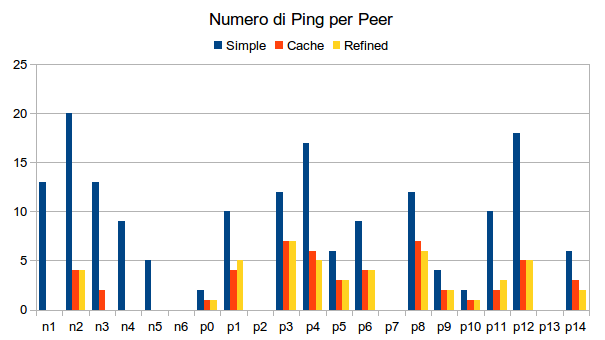
\includegraphics[height=3.5cm]{graph1ping.png}
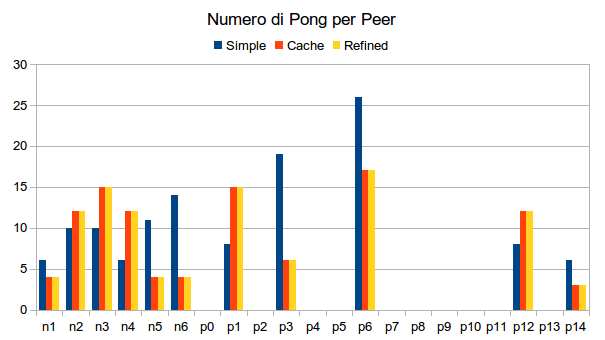
\includegraphics[height=3.5cm]{graph1pong.png}
\caption{\small{Grafici che mostrano il numero di ping e di pong che sono stati ricevuti da ogni peer della rete}}
\label{fig:peer}
\end{figure}

Si pu\`o notare come il numero di ping e di pong sia molto ridotto nel caso in cui si utilizzi il pong caching. Dai grafici si nota chiaramente che i peer che sono stati utilizzati per fare il bootstrap siano p1, p3 e p6 dato che hanno un numero di pong ricevuto molto elevato.

Si noti invece come alcuni peer non sono stati mai raggiunti da alcuni messaggi, questo \`e possibile in quanto la topologia della rete \`e molto sparsa e i test sono stati effettuati con un TTL basso, per cui molti messaggi vengono scartati prima di raggiungere i luoghi pi\`u lontani della rete.

Per il peer \textsf{p1} notiamo per\`o che il numero di pong \`e aumentato nel caso del pong caching, ci\`o pu\`o essere dovuto al fatto che il peer non \`e riuscito ad avere un numero di pong sufficienti a rispondere tramite la cache; ha quindi dovuto girare il messaggio di ping ed ha inoltre contattato i vicini per ricevere altri pong con cui riempire la cache.

\subsection{Numero di messagi totali}

Nei seguenti grafici si nota maggiormente il miglioramento delle performance indotto dal pong caching, in particolare sono stati effettuati test su reti da 10, 30 e 50 peer (sempre generate con probabilit\`a pari a 0.1) e si pu\`o notare chiaramente come vi sia una netta diminuzione del numero dei messaggi ricevuti.

\begin{figure}[ht]
\centering
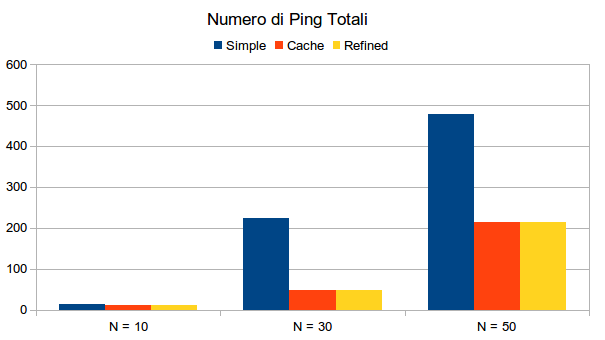
\includegraphics[height=3.5cm]{graph2ping.png}
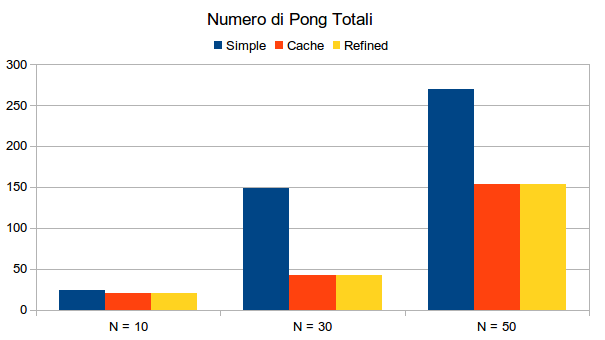
\includegraphics[height=3.5cm]{graph2pong.png}
\caption{\small{Grafici che mostrano il numero di ping e di pong che sono stati ricevuti in totale da tutti i peer della rete}}
\end{figure}

\begin{figure}[ht]
\centering
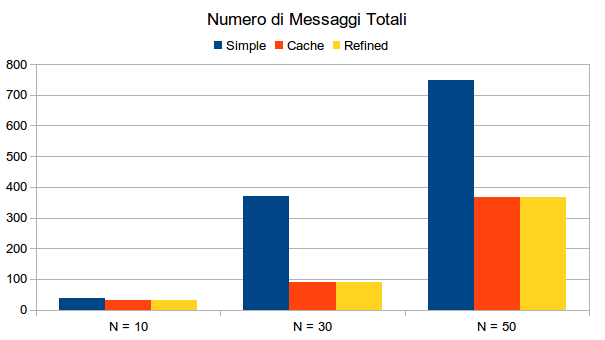
\includegraphics[height=3.5cm]{graph2total.png}

\caption{\small{Grafico che mostra il numero totale di messaggi che sono stati ricevuti da tutti i peer della rete}}
\end{figure}

Si noti come il caso refined abbia risultati identici al caso con la cache semplice, questo \`e dovuto al fatto che sono state effettuate le misurazioni dei messaggi al termine della fase di bootstrap. Dopo la fase di bootstrap la rete che non implementa il pong caching si stabilizza, mentre la rete con il pong caching semplice o refined continua ad inviare messaggi per effettuare il \emph{refresh} della cache.

\subsection{Messaggi legati al refresh}

Nel seguente grafico si vede come si evolve il numero dei messaggi ricevuti nel caso con il \emph{pong caching} semplice o refined: 

\begin{figure}[ht]
\centering
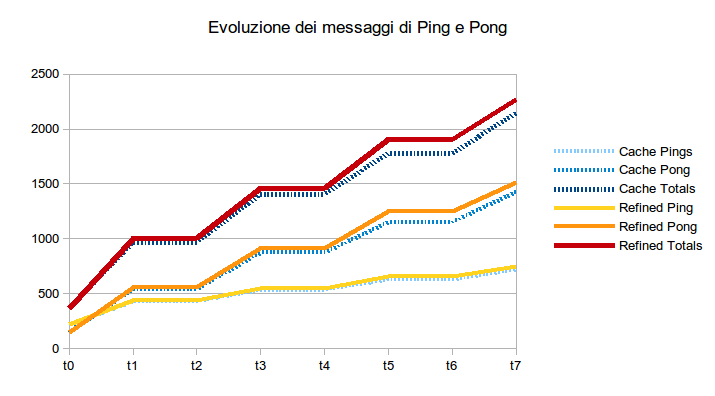
\includegraphics[height=7cm]{graph3.png}

\caption{\small{Grafico che mostra l'evoluzione del numero di messaggi nel tempo nella rete con \emph{pong caching} semplice e refined}}
\end{figure}

Si pu\`o notare come il numero dei messaggi cresca nel tempo. Il fatto di usare un \emph{pong caching} di tipo refined comporta un leggero aumento del numero dei messaggi, in quanto qualche pong memorizzato nella cache dei peer potrebbe scadere e portare i peer a non poter rispondere con i pong in cache (in quanto non risultano essere in numero sufficiente).

Questo fenomento si nota dal grafico in cui le linee continue (legate a casi refined) risultano avere valori leggermente maggiori. 

Non si pensi per\`o che il caso refined risulta peggiore, in quanto offre come risposte dei pong che riusciranno a far stabilire una connessione con probabilit\`a maggiore rispetto ai pong del caso semplice. Purtroppo questo fatto non si evince da questo grafico, ma si dovrebbe implementare all'interno della rete il fenomeno della caduta dei peer o dell'abbandono della rete.

\section{User Guide}
\label{sec:userguide}

Per installare il software \`e necessario posizionarsi all'interno della directory dove \`e contenuto il software ed invocare da terminale il comando
\begin{lstlisting}
ant
\end{lstlisting}

Nel caso si fosse interessati a conoscere i dettagli del processo di installazione, procedere con la lettura, altrimenti procedere dalla sezione relativa all'utilizzo del software.

\subsection{Installation}

Il software \`e corredato di un file \textbf{ant} (il file \texttt{build.xml}) che offre dei target per automatizzare il processo di compilazione e di configurazione del software.

In particolare \`e possibile inizializzare l'ambiente di lavoro utilizzando il comando
\begin{lstlisting}
ant init
\end{lstlisting}
che provvede a creare le cartelle necessarie per completare il processo di compilazione.

Per compilare il progetto \`e necessario eseguire il target 
\begin{lstlisting}
ant build
\end{lstlisting}
che provveder\`a ad invocare il compilatore \texttt{javac} per compilare i sorgenti presenti all'interno della cartella \texttt{src/}, i file \texttt{.class} generati si troveranno all'interno della cartella \texttt{bin/}. Il target \texttt{build} provvede ad invocare automaticamente il target \texttt{init}, per cui non \`e necessario invocare direttamente il target \texttt{init} a meno che non si sia interessati a configurare l'ambiente senza effettuare la compilazione.

Per pulire la cartella \texttt{bin/} al fine di avere un ambiente pulito per poter effettuare una nuova compilazione \`e possibile utilizzare il target
\begin{lstlisting}
ant clean
\end{lstlisting}

\`E infine possibile generare un file \texttt{jar} contenente tutti i file compilati. Per farlo \`e sufficiente invocare il target
\begin{lstlisting}
ant jar
\end{lstlisting}
Verr\`a generato un file chiamato \texttt{pingpong.jar} all'interno della cartella principale del software.
Per avviare il file \texttt{jar} \`e necessario invocare il comando
\begin{lstlisting}
java -jar pingpong.jar [parametri]
\end{lstlisting}

\subsection{Documentation}

Al fine di rendere il codice sorgente pi\`u comprensibile il software \`e stato corredato di documentazione. In particolare tutte le parti del codice che potrebbero risultare di difficile comprensione sono state commentate. Inoltre ogni funzione e classe del software \`e stata documentata con il formato \textsf {javadoc}, la documentazione generata pu\`o essere visionata all'interno della cartella \textsf{doc/} e pu\`o essere rigenerata utilizzando il comando
\begin{lstlisting}
ant javadoc
\end{lstlisting}

Per una comprensione organica del software si consiglia la lettura della seguente relazione nella sua interezza. La presente relazione viene rilasciata in Pdf ed in \LaTeX\ e pu\`o essere ricompilata utilizzando il comando\footnote{Si noti che tale target funziona solamente se installato il software \textsf{pdflatex} e se eseguito in ambiente UNIX}
\begin{lstlisting}
ant latex
\end{lstlisting}


\subsection{Software Usage}

Una volta compilato il software \`e possibile invocare il software tramite lo strumento \texttt{ant}, il software permette di essere invocato indicando alcuni parametri al fine di effettuare simulazioni con reti e protocolli differenti.

Il software pu\`o essere invocato tramite il comando
\begin{lstlisting}
ant <mode> [-Dpeer=filepeer] [-Dconn=fileconn] [-Ddyna=filedyna]
\end{lstlisting}


%%%%%%%%%%%%%%%%%%%%%
% TODO vanno inseriti i riferimenti
%%%%%%%%%%%%%%%%%%%%%

I parametri sono i seguenti:
\begin{description}
\item[-Dpeer=] Permette di impostare il file dei peer.
\item[-Dconn=] Permette di impostare il file delle connessioni.
\item[-Ddyna] Permette di impostare il file della dinamica.
\end{description}

Le modalit\`a sono le seguenti:
\begin{description}
\item[Simple] Esegue una simulazione in cui i peer della rete non implementano il \emph{pong caching},
\item[Cache] Esegue una simulazione in cui i peer della rete implementano il \emph{pong caching} semplice.
\item[Refined] Esegue una simulazione in cui i peer della rete implementano il \emph{refined pong caching}.
\end{description}

\paragraph{Generazione della rete}
\`E inoltre possibile effettuare la generazione di una coppia di file da utilizzare per effettuare la simulazione. Per generali \`e sufficiente invocare il comando:
\begin{lstlisting}
ant Generate [-Dn_peer=numberofpeer] [-Dt_conn=connectprob.ty]
\end{lstlisting}

Dove i parametri sono i seguenti:
\begin{description}
\item[-Dn\_peer=] Permette di impostare il numero dei peer che faranno parte della rete simulata,
\item[-Dt\_conn=] Permette di impostare la probabilit\`a che esista una connesione fra due generici peer.
\end{description}

\section{Future Improvements}

Sono possibili ulteriori miglioramenti al software che potrebbero essere implementati in versioni future:

\begin{itemize}
\item Utilizzare i campi \textsf{sharedfiles} e \textsf{sharedbytes} all'interno dei \textsf{Message} in modo che i peer che stanno effettuando il bootstrap possano effettuare una scelta pi\`u oculata dei peer a cui connettersi al fine di favorire i peer che stanno condividendo pi\`u files e di scoraggiare i peer che stanno condividendo poco.

\item Aggiornare le classi \textsf{Message} e \textsf{Peer} per permettere la ricezione e l'invio di messaggi di \textsf{QUERY}, \textsf{QUERY\_HIT}, etc...

\item Aggiornare la funzione \textsf{getPongs} di \textsf{PongCache} in modo che si riceva un insieme di pong con valori di HOPS differenti, in modo da permettere al peer che si sta connettendo di connettersi a peer che sono sia vicini, che distanti.

\item Implementare la possibilit\`a che un nodo abbandoni la rete spontaneamente oppure non spontaneamente (per esempio in seguito ad un guasto della rete).

\item Inserire un timer che risponda ad un ping solamente se non sono stati ricevuti ping sulla stessa connessione per un certo tempo (ad esempio 1 secondo)\footnote{Secondo quanto definito nell'RFC di Gnutella: \url{http://rfc-gnutella.sourceforge.net/src/rfc-0_6-draft.html}}.

\item Inserire una dimensione massima della cache, in modo da non sovraccaricare la memoria dei peer.
\end{itemize}

%%%%%%%%%%%%%%%%%
% Si mette?
%%%%%%%%%%%%%%%%%

\section{Licence}

\small{Tutto il codice sorgente scritto viene rilasciato sotto licenza Gnu GPL - General Public Licence versione 3, ognuno \`e libero di modificare e di distribuire il codice sorgente entro i termini di tale licenza.
Tale licenza pu\`o essere consultata all'indirizzo:

http://www.gnu.org/copyleft/gpl.html

\begin{verbatim}
Copyright (C)  2013  Nicola Corti.
Permission is granted to copy, distribute and/or modify this document
under the terms of the GNU Free Documentation License, Version 1.3
or any later version published by the Free Software Foundation;
with no Invariant Sections, no Front-Cover Texts, and no Back-Cover Texts.
\end{verbatim}
Per qualsiasi problema \`e possibile contattare lo sviluppatore all'indirizzo e-mail \texttt{cortin [at] cli.di.unipi.it}.
}
\end{document}
